\documentclass[11pt]{article}
\usepackage{amsthm,amsmath,amsfonts,environ,amssymb}
\usepackage{bm}
\usepackage[sc]{mathpazo}
\linespread{1.05}         % Palladio needs more leading (space between lines).
\usepackage[T1]{fontenc}
\usepackage{calc}
\usepackage[top=1in, bottom=1in, left=0.75in, right=0.75in]{geometry}
\usepackage{algcompatible}
\usepackage{graphics}
\usepackage{graphicx}
\usepackage{url}
\usepackage{xcolor}
\usepackage{hyperref}
\usepackage{listings}
\usepackage{enumitem}

% Listing code style: feel free to modify for a different look.
\definecolor{codegreen}{rgb}{0,0.6,0}
\definecolor{codepurple}{rgb}{0.58,0,0.82}
\lstdefinestyle{codestyle}{
    commentstyle=\color{codegreen},
    keywordstyle=\color{blue},
    numberstyle=\tiny\color{gray},
    stringstyle=\color{codepurple},
    basicstyle=\fontfamily{pcr}\selectfont\footnotesize,
    breakatwhitespace=false,
    breaklines=true,
    captionpos=b,
    keepspaces=true,
    numbers=left,
    numbersep=5pt,
    showspaces=false,
    showstringspaces=false,
    showtabs=false,
    tabsize=2
}
\lstset{style=codestyle}
  % Packages and definitions specified here.
\usepackage{fontawesome5}

%*******************************************************************************
% Theorem Environments
%*******************************************************************************
\newtheorem{theorem}{Theorem}
\newtheorem{proposition}{Proposition}
\newtheorem{lemma}{Lemma}
\newtheorem{corollary}{Corollary}
\newtheorem{claim}{Claim}
\newtheorem{definition}{Definition}
\newtheorem{assumption}{Assumption}
\newtheorem{remark}{Remark}

%*******************************************************************************
% Dynamics and Uncertainty
%*******************************************************************************
\newcommand{\reals}{\mathbb{R}}
\newcommand{\naturals}{\mathbb{N}} 
\newcommand{\rationals}{\mathbb{Q}}
\newcommand{\integers}{\mathbb{Z}}
\newcommand{\compl}{\mathsf{c}}
\newcommand{\bdry}{{\partial}}

\newcommand{\stateset}{{\mathcal{X}}}
\newcommand{\obsset}{{\mathcal{Y}}}
\newcommand{\ctrlset}{{\mathcal{U}}}
\newcommand{\dstbset}{{\mathcal{D}}}
\newcommand{\trajset}{{\mathbb{X}}}
\newcommand{\ctrsigset}{{\mathbb{U}}}
\newcommand{\dstbsigset}{{\mathbb{D}}}

\newcommand{\dyn}{{f}}
\newcommand{\tvar}{{t}}
\newcommand{\taux}{{\tau}}
\newcommand{\horizon}{{T}}

\newcommand{\state}{{x}}
\newcommand{\ctrl}{{u}}
\newcommand{\dstb}{{d}}

\newcommand{\traj}{{\mathbf{\state}}}
\newcommand{\csig}{{\mathbf{\ctrl}}}
\newcommand{\dsig}{{\mathbf{\dstb}}}

%*******************************************************************************
% Optimal control and dynamic games
%*******************************************************************************
\newcommand{\outcome}{{J}}
\newcommand{\valfunc}{{V}}
\newcommand{\qfunc}{{Q}}

\newcommand{\policy}{{\pi}}
\newcommand{\feedback}{{K}}
\newcommand{\strat}{{\bm\gamma}}
\newcommand{\cstrat}{{\bm{\upsilon}}}
\newcommand{\dstrat}{{\bm{\delta}}}

%*******************************************************************************
% Safety analysis and safety filters
%*******************************************************************************
\newcommand{\safeset}{{\Omega}}
\newcommand{\safe}{\text{\tiny{\faShield*}}}

\newcommand{\target}{{\mathcal{T}}}
\newcommand{\failure}{{\mathcal{F}}}
\newcommand{\reach}{{\mathcal{R}}}
\newcommand{\reachavoid}{{\mathcal{RA}}}

\newcommand{\inevitable}[1]{{#1}^-}
\newcommand{\enforceable}[1]{{#1}^+}
\newcommand{\forward}[1]{\overrightarrow{#1}}
\newcommand{\backward}[1]{\overleftarrow{#1}}

\newcommand{\invkernel}{{\text{\textnormal{Inv}}}}
\newcommand{\viabkernel}{{\text{\textnormal{Viab}}}}
\newcommand{\disckernel}{{\text{\textnormal{Disc}}}}
  % Conveniently define (and quickly redefine!) notation here.
\usepackage{subcaption}

% ---- Local shorthands for this problem set -----------------------------------
\newcommand{\Usig}{\ctrsigset_{\tvar_0}^{\tvar}}                 % admissible control signals on [t0,t]
\newcommand{\trj}[1]{\state_{\state_0,\tvar_0}(#1)}                 % autonomous trajectory
\newcommand{\trju}[2]{\state^{#1}_{\state_0,\tvar_0}(#2)}          % controlled trajectory
\newcommand{\BRS}[1]{\backward{\reach}_{#1}(\target)}               % backward-reachable set
\newcommand{\BRT}[2]{\backward{\reach}_{[\tvar_0,#1]}(#2)}          % backward-reachable tube
\newcommand{\RAT}[1]{\backward{\reachavoid}_{[\tvar_0,#1]}(\target,\failure)}
\newcommand{\eBRT}[2]{\enforceable{\backward{\reach}}_{[\tvar_0,#1]}(#2)}
\newcommand{\iBRT}[2]{\inevitable{\backward{\reach}}_{[\tvar_0,#1]}(#2)}
\newcommand{\eRAT}[1]{\enforceable{\backward{\reachavoid}}_{[\tvar_0,#1]}(\target,\failure)}
\newcommand{\Safe}[2]{\safeset_{[\tvar_0,#1]}(#2)}
\newcommand{\eBRTinf}[1]{\enforceable{\backward{\reach}}_{[\tvar_0,\infty)}(#1)}
\newcommand{\iBRTinf}[1]{\inevitable{\backward{\reach}}_{[\tvar_0,\infty)}(#1)}
\newcommand{\Mone}{\mathcal{M}_1}
\newcommand{\Mtwo}{\mathcal{M}_2}
\newcommand{\Mthree}{\mathcal{M}_3}
\newcommand{\TRUE}{\textbf{True.}}
\newcommand{\FALSE}{\textbf{False.}}

\title{\large ECE 532/COS 572/MAE 572/ROB 532 \\[-1mm]
       \LARGE Safety-Critical Robotics and AI \\[1mm]
       \large Problem Set 1}
\author{Yixun Hu}
\date{\today}

\begin{document}
\maketitle

%===============================================================================
\section*{Problem 1: Reachability Analysis}
%===============================================================================

\noindent\textbf{Conventions.}
For the autonomous system, $\trj{\cdot}$ denotes the unique trajectory that starts from
$\state_0$ at time $\tvar_0$. For the controlled system, $\trju{\ctrl}{\cdot}$ denotes the
trajectory generated by the control signal $\ctrl(\cdot)\in\Usig$, the set of admissible control
signals on $[\tvar_0,\tvar]$, which we assume to be nonempty. Trajectories are continuous in
time. Since ``$A\subseteq B$'' means ``$\state_0\in A \Rightarrow \state_0\in B$'', each proof
below takes an arbitrary point of the left-hand set and exhibits the witnesses required by the
definition of the right-hand set, and each counterexample exhibits a point that lies in the
left-hand set but not in the right-hand set.

\subsection*{Part 1: autonomous system $\dot\state=\dyn(\state)$}

\begin{enumerate}[label=(\alph*), itemsep=3pt]

\item \TRUE\
Let $\state_0\in\BRS{\tvar}$, i.e.\ $\trj{\tvar}\in\target$. Choose $\taux:=\tvar$. Then
$\taux\in[\tvar_0,\tvar]$ and $\trj{\taux}\in\target$, which is exactly the defining condition of
$\BRT{\tvar}{\target}$; hence $\state_0\in\BRT{\tvar}{\target}$. In words, the tube collects the
states that visit $\target$ at \emph{some} time in the horizon, in particular those that are in
$\target$ exactly at the final time.

\item \TRUE\
Let $\state_0\in\BRT{\tvar}{\target}$: there is $\taux\in[\tvar_0,\tvar]$ with
$\trj{\taux}\in\target$. Because $\tvar<\tvar'$ we have $[\tvar_0,\tvar]\subseteq[\tvar_0,\tvar']$,
so the same $\taux$ satisfies $\taux\in[\tvar_0,\tvar']$ and $\trj{\taux}\in\target$; therefore
$\state_0\in\BRT{\tvar'}{\target}$. Backward-reachable tubes are monotone (non-decreasing) in the
horizon.

\item \FALSE\
The backward-reachable \emph{set} only constrains the state at time $\tvar$; it does not care
whether the trajectory passed through $\failure$ on the way. Counterexample ($n=1$):
\[
\dot\state = 1,\qquad \tvar_0=0,\quad \tvar=2,\qquad \target=\{2\},\quad \failure=\{1\}
\]
(both nonempty and disjoint). From $\state_0=0$ the trajectory is $\trj{\taux}=\taux$, so
$\trj{2}=2\in\target$ and $\state_0\in\BRS{2}$. However, the only time in $[0,2]$ at which the
trajectory is in $\target$ is $\taux=2$, and for $s=1\in[\tvar_0,\taux]$ we have
$\trj{1}=1\in\failure$. The avoid condition fails for the only admissible $\taux$, so
$\state_0\notin\RAT{2}$. Hence $\BRS{\tvar}\not\subseteq\RAT{\tvar}$ in general.

\item \TRUE\
Let $\state_0\in\RAT{\tvar}$. By definition there is $\taux\in[\tvar_0,\tvar]$ such that
$\trj{\taux}\in\target$ \emph{and} $\trj{s}\notin\failure$ for all $s\in[\tvar_0,\taux]$. The
first conjunct, with the same witness $\taux$, is precisely the defining condition of
$\BRT{\tvar}{\target}$; hence $\state_0\in\BRT{\tvar}{\target}$. Dropping a conjunct from a
membership condition can only enlarge the set, so the reach-avoid tube is always contained in the
reach tube.

\end{enumerate}

\subsection*{Part 2: controlled system $\dot\state=\dyn(\state,\ctrl)$}

\begin{enumerate}[label=(\alph*), itemsep=3pt]

\item \TRUE\
Let $\state_0\in\iBRT{\tvar}{\target}$: for \emph{every} $\ctrl(\cdot)\in\Usig$ there is
$\taux_{\ctrl}\in[\tvar_0,\tvar]$ with $\trju{\ctrl}{\taux_{\ctrl}}\in\target$. Since
$\Usig\neq\emptyset$ we may fix any particular $\bar\ctrl(\cdot)\in\Usig$; then
$\taux_{\bar\ctrl}\in[\tvar_0,\tvar]$ and $\trju{\bar\ctrl}{\taux_{\bar\ctrl}}\in\target$, so the
pair $(\bar\ctrl,\taux_{\bar\ctrl})$ witnesses $\state_0\in\eBRT{\tvar}{\target}$. In short,
``for all $\ctrl$'' implies ``there exists $\ctrl$'' because the set of admissible controls is
nonempty: if reaching $\target$ cannot be avoided, then it can certainly be enforced.

\item \FALSE\
The enforceable reach-avoid tube is
\[
\eRAT{\tvar} := \bigl\{\state_0\in\reals^n :\ \exists\,\ctrl(\cdot)\in\Usig,\ \exists\,\taux\in[\tvar_0,\tvar],\
\trju{\ctrl}{\taux}\in\target \ \wedge\ \forall s\in[\tvar_0,\taux],\ \trju{\ctrl}{s}\notin\failure\bigr\}.
\]
The intersection $\eBRT{\tvar}{\target}\cap\Safe{\tvar}{\failure}$ allows \emph{one} control to
reach $\target$ and a \emph{different} control to avoid $\failure$, whereas $\eRAT{\tvar}$ requires
a \emph{single} control to do both. Counterexample ($n=1$):
\[
\dot\state=\ctrl,\quad \ctrl\in[-1,1],\qquad \tvar_0=0,\quad \tvar=2,\qquad
\target=\{2\},\quad \failure=\{1\},\qquad \state_0=0.
\]
\begin{itemize}[itemsep=0pt]
\item $\state_0\in\eBRT{2}{\target}$: with $\ctrl\equiv1$, $\trju{\ctrl}{\taux}=\taux$, so
      $\trju{\ctrl}{2}=2\in\target$.
\item $\state_0\in\Safe{2}{\failure}$: with $\ctrl\equiv0$, $\trju{\ctrl}{\taux}\equiv0\notin\failure$
      for all $\taux\in[0,2]$.
\item $\state_0\notin\eRAT{2}$: if some control satisfies $\trju{\ctrl}{\taux}=2$ for some $\taux$,
      the (continuous) trajectory goes from $0$ to $2$, so by the intermediate value theorem
      $\trju{\ctrl}{s}=1\in\failure$ for some $s\in(0,\taux)$. The avoid condition therefore fails
      for every candidate pair $(\ctrl,\taux)$.
\end{itemize}
Hence $\eBRT{\tvar}{\target}\cap\Safe{\tvar}{\failure}\not\subseteq\eRAT{\tvar}$, and the equality
is false. (The reverse inclusion fails in general as well, because $\eRAT{\tvar}$ only asks to avoid
$\failure$ \emph{until} $\target$ is reached, while $\Safe{\tvar}{\failure}$ asks to avoid it over
the whole horizon. With $\dot\state=1+\ctrl$, $\ctrl\in[-\tfrac12,\tfrac12]$, $\tvar_0=0$, $\tvar=10$,
$\target=\{1\}$, $\failure=\{2\}$, the state $\state_0=0$ lies in $\eRAT{10}$, since $\ctrl\equiv0$
reaches $1$ at $\taux=1$ without touching $2$, but not in $\Safe{10}{\failure}$, since
$\dot\state\ge\tfrac12$ forces $\trju{\ctrl}{4}\ge2$ and thus every trajectory crosses $2$ before
time $4<10$.)

\item \FALSE\
Only the inclusion ``$\subseteq$'' holds in general.

\emph{Proof of $\Safe{\tvar}{\failure_1\cup\failure_2}\subseteq\Safe{\tvar}{\failure_1}\cap\Safe{\tvar}{\failure_2}$.}
If $\state_0\in\Safe{\tvar}{\failure_1\cup\failure_2}$ with witness $\ctrl(\cdot)$, then
$\trju{\ctrl}{\taux}\notin\failure_1\cup\failure_2$ for all $\taux\in[\tvar_0,\tvar]$, i.e.\
$\trju{\ctrl}{\taux}\notin\failure_1$ and $\trju{\ctrl}{\taux}\notin\failure_2$. The same
$\ctrl(\cdot)$ therefore witnesses both $\state_0\in\Safe{\tvar}{\failure_1}$ and
$\state_0\in\Safe{\tvar}{\failure_2}$.

\emph{Counterexample to ``$\supseteq$''.} The controls that avoid $\failure_1$ and $\failure_2$ may be
different, and no single control may avoid both. Take $n=2$, $\state=(\state_1,\state_2)$,
\[
\dot\state_1=1,\quad \dot\state_2=\ctrl,\quad \ctrl\in[-1,1],\qquad \tvar_0=0,\quad \tvar=1,\qquad
\state_0=(0,0),
\]
\[
\failure_1=\{(1,\state_2):\state_2\ge0\},\qquad
\failure_2=\{(1,\state_2):\state_2\le0\},\qquad
\failure_1\cup\failure_2=\{(1,\state_2):\state_2\in\reals\}.
\]
\begin{itemize}[itemsep=0pt]
\item $\state_0\in\Safe{1}{\failure_1}$: with $\ctrl\equiv-1$ the trajectory is $(\taux,-\taux)$. It has
      $\state_1=1$ only at $\taux=1$, where $\state_2=-1<0$, so it never enters $\failure_1$.
\item $\state_0\in\Safe{1}{\failure_2}$: symmetrically, $\ctrl\equiv+1$ gives $(\taux,\taux)$, which
      never enters $\failure_2$.
\item $\state_0\notin\Safe{1}{\failure_1\cup\failure_2}$: $\state_1(\taux)=\taux$ regardless of the
      control, so at $\taux=1\in[0,1]$ every trajectory satisfies
      $\trju{\ctrl}{1}=(1,\state_2(1))\in\failure_1\cup\failure_2$.
\end{itemize}
Thus $\Safe{\tvar}{\failure_1}\cap\Safe{\tvar}{\failure_2}\supsetneq\Safe{\tvar}{\failure_1\cup\failure_2}$
in general: being able to dodge each hazard separately does not imply being able to dodge both at
once. Taking complements (note $\reals^n\setminus\Safe{\tvar}{\failure}=\iBRT{\tvar}{\failure}$),
the inevitable BRT of a union of failure sets can be \emph{strictly larger} than the union of the
individual inevitable BRTs; Problem~3 exhibits exactly this effect.

\end{enumerate}

%===============================================================================
\section*{Problem 2: 1-D Reachable Sets}
%===============================================================================

\noindent\textbf{Setup.}
The control signals $\ctrl(\cdot)$ are measurable with values in $[-1,1]$, and the \emph{all-time}
tubes are the tubes over the horizon $[\tvar_0,\infty)$:
\begin{align*}
\eBRTinf{\mathcal M}&=\{\state_0:\ \exists\,\ctrl(\cdot),\ \exists\,\taux\ge\tvar_0,\ \trju{\ctrl}{\taux}\in\mathcal M\},\\
\iBRTinf{\mathcal M}&=\{\state_0:\ \forall\,\ctrl(\cdot),\ \exists\,\taux_{\ctrl}\ge\tvar_0,\ \trju{\ctrl}{\taux_{\ctrl}}\in\mathcal M\}.
\end{align*}
Both tubes contain $\mathcal M$ itself (take $\taux=\tvar_0$), and the inevitable tube is contained
in the enforceable one (Problem~1.2(a)). Without loss of generality $\tvar_0=0$. In every
``inevitable'' claim below the hitting time is bounded uniformly over the controls, so the answers
are unchanged if the all-time tubes are instead defined as $\bigcup_{\tvar\ge\tvar_0}$ of the
finite-horizon tubes. The sets of interest are
$\Mone=[\tfrac12,2]$ and $\Mtwo=[-3,-\tfrac12]\cup[2,3]$.

\subsection*{Part 1: stable dynamics $\dot\state=-\state+\ctrl$}

Since $\dot\state\in[-\state-1,\,-\state+1]$: for $\state>1$ every control gives $\dot\state<0$, for
$\state<-1$ every control gives $\dot\state>0$, and for $\state\in[-1,1]$ the controller can hold the
state ($\ctrl\equiv\state$), push it up ($\ctrl\equiv1$) or push it down ($\ctrl\equiv-1$). The
extreme closed-loop trajectories are
\begin{align*}
\ctrl\equiv1:&\quad \state(\tvar)=1+(\state_0-1)e^{-\tvar}\qquad(\text{monotone to }1),\\
\ctrl\equiv-1:&\quad \state(\tvar)=-1+(\state_0+1)e^{-\tvar}\qquad(\text{monotone to }-1),
\end{align*}
and by the comparison principle every trajectory is sandwiched between them:
\begin{equation}\label{eq:stable-bounds}
-1+(\state_0+1)e^{-\tvar}\ \le\ \state(\tvar)\ \le\ 1+(\state_0-1)e^{-\tvar},
\quad\text{hence}\quad
\min(\state_0,-1)\le\state(\tvar)\le\max(\state_0,1).
\end{equation}
The drift pulls every state toward $[-1,1]$ and no control can move the state \emph{away} from the
origin past $\pm1$.

\begin{enumerate}[label=(\alph*), itemsep=3pt]
\item $\Mone=[\tfrac12,2]$.

\emph{Enforceable tube:} $\eBRTinf{\Mone}=\reals$.
For $\state_0\in\Mone$ take $\taux=0$. For $\state_0>2$, every control gives
$\dot\state\le-\state+1\le-1$ as long as $\state\ge2$, so the state decreases and hits $2\in\Mone$ no
later than $\taux=\state_0-2$ (for \emph{every} control). For $\state_0<\tfrac12$, the control
$\ctrl\equiv1$ gives $\state(\tvar)=1+(\state_0-1)e^{-\tvar}\uparrow1$, which crosses $\tfrac12$ at
the finite time $\taux=\ln\bigl(2(1-\state_0)\bigr)$.

\emph{Inevitable tube:} $\iBRTinf{\Mone}=[\tfrac12,\infty)$.
Points of $\Mone$ and points $\state_0>2$ are inevitable by the argument above. For
$\state_0<\tfrac12$ the control $\ctrl\equiv-1$ gives $\state(\tvar)=-1+(\state_0+1)e^{-\tvar}$,
which stays between $\state_0$ and $-1$ for all times, hence $\state(\tvar)\le\max(\state_0,-1)<\tfrac12$
and the trajectory never enters $\Mone$.

\item $\Mtwo=[-3,-\tfrac12]\cup[2,3]$.

\emph{Enforceable tube:} $\eBRTinf{\Mtwo}=\reals$.
For $\state_0\in\Mtwo$ take $\taux=0$. For $\state_0>3$, every control gives
$\dot\state\le-\state+1\le-2$ while $\state\ge3$, so the state hits $3\in\Mtwo$ no later than
$\taux=(\state_0-3)/2$; symmetrically, for $\state_0<-3$ every control gives
$\dot\state\ge-\state-1\ge2$ while $\state\le-3$, so the state hits $-3\in\Mtwo$ no later than
$\taux=(-3-\state_0)/2$. For $\state_0\in(-\tfrac12,2)$ the control $\ctrl\equiv-1$ gives
$\state(\tvar)=-1+(\state_0+1)e^{-\tvar}\downarrow-1$, which crosses $-\tfrac12$ at the finite time
$\taux=\ln\bigl(2(\state_0+1)\bigr)$.

\emph{Inevitable tube:} $\iBRTinf{\Mtwo}=(-\infty,-\tfrac12]\cup[2,\infty)$.
Points of $\Mtwo$ and points with $\state_0>3$ or $\state_0<-3$ are inevitable by the argument above.
The remaining points $\state_0\in(-\tfrac12,2)$ can avoid $\Mtwo$ forever: if $\state_0\in(-\tfrac12,1]$,
the constant control $\ctrl\equiv\state_0$ (admissible since $|\state_0|\le1$) holds
$\state(\tvar)\equiv\state_0\notin\Mtwo$; if $\state_0\in(1,2)$, the control $\ctrl\equiv1$ gives
$\state(\tvar)=1+(\state_0-1)e^{-\tvar}\in(1,\state_0]\subset(1,2)$ for all times.
\end{enumerate}

\subsection*{Part 2: unstable dynamics $\dot\state=\state+\ctrl$}

Now $\dot\state\in[\state-1,\,\state+1]$: for $\state>1$ every control gives $\dot\state>0$, for
$\state<-1$ every control gives $\dot\state<0$, and on $(-1,1)$ the controller can hold the state
($\ctrl\equiv-\state$) or steer it in either direction. The extreme trajectories are
\[
\ctrl\equiv1:\ \state(\tvar)=-1+(\state_0+1)e^{\tvar},\qquad
\ctrl\equiv-1:\ \state(\tvar)=1+(\state_0-1)e^{\tvar},
\]
and every trajectory satisfies
\begin{equation}\label{eq:unstable-bounds}
1+(\state_0-1)e^{\tvar}\ \le\ \state(\tvar)\ \le\ -1+(\state_0+1)e^{\tvar}.
\end{equation}
Consequently: if $\state_0>1$ then $\state(\tvar)>\state_0$ for all $\tvar>0$ and
$\state(\tvar)\to\infty$ for every control; if $\state_0\le-1$ then $\state(\tvar)\le-1$ for all
times (and $\state(\tvar)\to-\infty$ if $\state_0<-1$); the drift now pushes the state \emph{away}
from the origin, and the controller only has authority inside $[-1,1]$.

\begin{enumerate}[label=(\alph*), itemsep=3pt]
\item $\Mone=[\tfrac12,2]$.

\emph{Enforceable tube:} $\eBRTinf{\Mone}=(-1,2]$.
For $\state_0\in\Mone$ take $\taux=0$. For $\state_0\in(-1,\tfrac12)$ the control $\ctrl\equiv1$
gives $\state(\tvar)=-1+(\state_0+1)e^{\tvar}\uparrow\infty$, which crosses $\tfrac12$ at the finite
time $\taux=\ln\bigl(\tfrac{3}{2(\state_0+1)}\bigr)$. For $\state_0>2$, \eqref{eq:unstable-bounds}
gives $\state(\tvar)>\state_0>2$ for every control, and for $\state_0\le-1$ it gives
$\state(\tvar)\le-1<\tfrac12$ for every control; neither can ever reach $\Mone$.

\emph{Inevitable tube:} $\iBRTinf{\Mone}=[\tfrac12,2]=\Mone$.
Points outside $(-1,2]$ are not even enforceable. For $\state_0\in(-1,\tfrac12)$ the control
$\ctrl\equiv-1$ gives $\state(\tvar)=1+(\state_0-1)e^{\tvar}$, which is decreasing because
$\state_0<1$, so $\state(\tvar)\le\state_0<\tfrac12$ forever and $\Mone$ is avoided.

\item $\Mtwo=[-3,-\tfrac12]\cup[2,3]$.

\emph{Enforceable tube:} $\eBRTinf{\Mtwo}=[-3,3]$.
For $\state_0\in\Mtwo$ take $\taux=0$. For $\state_0\in(-\tfrac12,2)$ the control $\ctrl\equiv1$
gives $\state(\tvar)=-1+(\state_0+1)e^{\tvar}\uparrow\infty$, which crosses $2\in\Mtwo$ in finite
time. For $\state_0>3$ we have $\state(\tvar)>\state_0>3$, and for $\state_0<-3$ we have
$\state(\tvar)<\state_0<-3$, for every control and all $\tvar>0$; $\Mtwo$ is never reached.

\emph{Inevitable tube:} $\iBRTinf{\Mtwo}=[-3,-\tfrac12]\cup(1,3]$.
For $\state_0\in(1,2)$, \eqref{eq:unstable-bounds} gives $\state(\tvar)\ge1+(\state_0-1)e^{\tvar}$
for every control; the right-hand side equals $2$ at $\tvar=\ln\bigl(1/(\state_0-1)\bigr)$, so the
continuous trajectory, which starts below $2$, crosses $2\in\Mtwo$ no later than that time. Thus
$(1,2)\subset\iBRTinf{\Mtwo}$ even though $(1,2)\cap\Mtwo=\emptyset$: the unstable drift drags these
states into $[2,3]$. For $\state_0\in(-\tfrac12,1]$ the constant control $\ctrl\equiv-\state_0$
(admissible since $|\state_0|\le1$) holds $\state(\tvar)\equiv\state_0\notin\Mtwo$. Points with
$|\state_0|>3$ are not enforceable.
\end{enumerate}

\begin{table}[h]
\centering
\begin{tabular}{lcc}
\hline
 & stable $\dot\state=-\state+\ctrl$ & unstable $\dot\state=\state+\ctrl$ \\
\hline
$\eBRTinf{\Mone}$ & $\reals$ & $(-1,2]$ \\
$\iBRTinf{\Mone}$ & $[\tfrac12,\infty)$ & $[\tfrac12,2]$ \\
$\eBRTinf{\Mtwo}$ & $\reals$ & $[-3,3]$ \\
$\iBRTinf{\Mtwo}$ & $(-\infty,-\tfrac12]\cup[2,\infty)$ & $[-3,-\tfrac12]\cup(1,3]$ \\
\hline
\end{tabular}
\caption{Summary of the all-time backward-reachable tubes in Problem 2.}
\end{table}

\subsection*{Part 3: a set that is strictly easier to reach with the unstable dynamics}

Take $\Mthree:=[2,\infty)$.
\begin{itemize}[itemsep=2pt]
\item \emph{Stable dynamics:} $\eBRTinf{\Mthree}=[2,\infty)=\Mthree$. Points of $\Mthree$ are
      trivially included. For $\state_0<2$, \eqref{eq:stable-bounds} gives
      $\state(\tvar)\le\max(\state_0,1)<2$ for every control and every time, so $\Mthree$ is never
      reached: bounded controls cannot overcome the drift toward the origin once $\state>1$.
\item \emph{Unstable dynamics:} $\eBRTinf{\Mthree}=(-1,\infty)$. For $\state_0>-1$ the control
      $\ctrl\equiv1$ gives $\state(\tvar)=-1+(\state_0+1)e^{\tvar}\uparrow\infty$, which crosses $2$
      in finite time. For $\state_0\le-1$, \eqref{eq:unstable-bounds} gives $\state(\tvar)\le-1$
      for every control, so $\Mthree$ is unreachable.
\end{itemize}
Hence $(-1,\infty)\supsetneq[2,\infty)$: the enforceable tube under the unstable dynamics strictly
contains the one under the stable dynamics. Intuitively, the controller can nudge any state in
$(-1,1)$ slightly past $1$ and then let the instability carry it arbitrarily far, whereas the stable
drift pulls everything back toward $[-1,1]$, so a far-away target can only be reached from states
that are already beyond it. Any $\Mthree=[a,\infty)$ with $a\ge1$ works (as does the symmetric
$(-\infty,-a]\cup[a,\infty)$, whose enforceable tubes are itself and $\reals$, respectively). Bounded
targets cannot work: for $\Mthree=[a,b]$ with $a>1$ the two enforceable tubes are $[a,\infty)$ and
$(-1,b]$, and neither contains the other, since the stable drift lets far-away states fall back onto
the target while the unstable drift never lets states beyond the target come back.

%===============================================================================
\section*{Problem 3: Backward Reachable Set -- Programming}
%===============================================================================

\subsection*{Implementation}

The robot advances one row per step and can shift by at most one column,
$(x_{\tvar+1},y_{\tvar+1})=(x_\tvar+\ctrl_\tvar,\,y_\tvar+1)$ with $\ctrl_\tvar\in\{-1,0,1\}$;
landing on an obstacle cell is a failure. \lstinline{get_successors} returns the cells reachable in
one step (moves that would leave the grid are treated as inadmissible; for the obstacle layout in
this problem the tube never touches the side walls, so this choice does not affect the results).
\lstinline{calculate_inevitable_brt} computes the inevitable BRT of the failure set $\failure$ by
the fixed-point iteration
\[
\inevitable{\backward{\reach}}_{0}=\failure,\qquad
\inevitable{\backward{\reach}}_{k+1}=\inevitable{\backward{\reach}}_{k}\ \cup\
\bigl\{\state:\ \dyn(\state,\ctrl)\in\inevitable{\backward{\reach}}_{k}\ \text{for \emph{all}}\ \ctrl\in\{-1,0,1\}\bigr\},
\]
i.e.\ a cell is added when every admissible control leads into the current set (no escape route),
and the iteration stops when a sweep adds nothing. Because $y$ increases by one every step, only the
rows below the highest obstacle row can ever collide, and the loop converges after at most that many
sweeps. The complement of the resulting set is the (all-time) safe set $\safeset(\failure)$; this is
the discrete-time, finite-state counterpart of the HJ reachability formulation
in~\cite{bansal2017hamilton}.

\lstinputlisting[language=Python]{get_successors.py}
\lstinputlisting[language=Python]{calculate_inevitable_brt.py}

\subsection*{Results}

\noindent\begin{minipage}{\linewidth}
Figure~\ref{fig:brt} shows the grid world and the three inevitable BRTs produced by the notebook.
With obstacle~1 occupying columns $\{2,3,4\}$ of row~5 and obstacle~2 occupying columns $\{5,6\}$:
\begin{center}
\begin{tabular}{ll}
\hline
failure set & inevitable BRT minus the obstacle cells \\
\hline
obstacle 1 (width 3) & $\{(3,4)\}$ \\
obstacle 2 (width 2) & $\emptyset$ \\
both obstacles (width 5) & $\{(3,4),(4,4),(5,4),(4,3)\}$ \\
\hline
\end{tabular}
\end{center}
\end{minipage}

\begin{figure}[h]
\centering
\begin{subfigure}[t]{0.42\linewidth}
  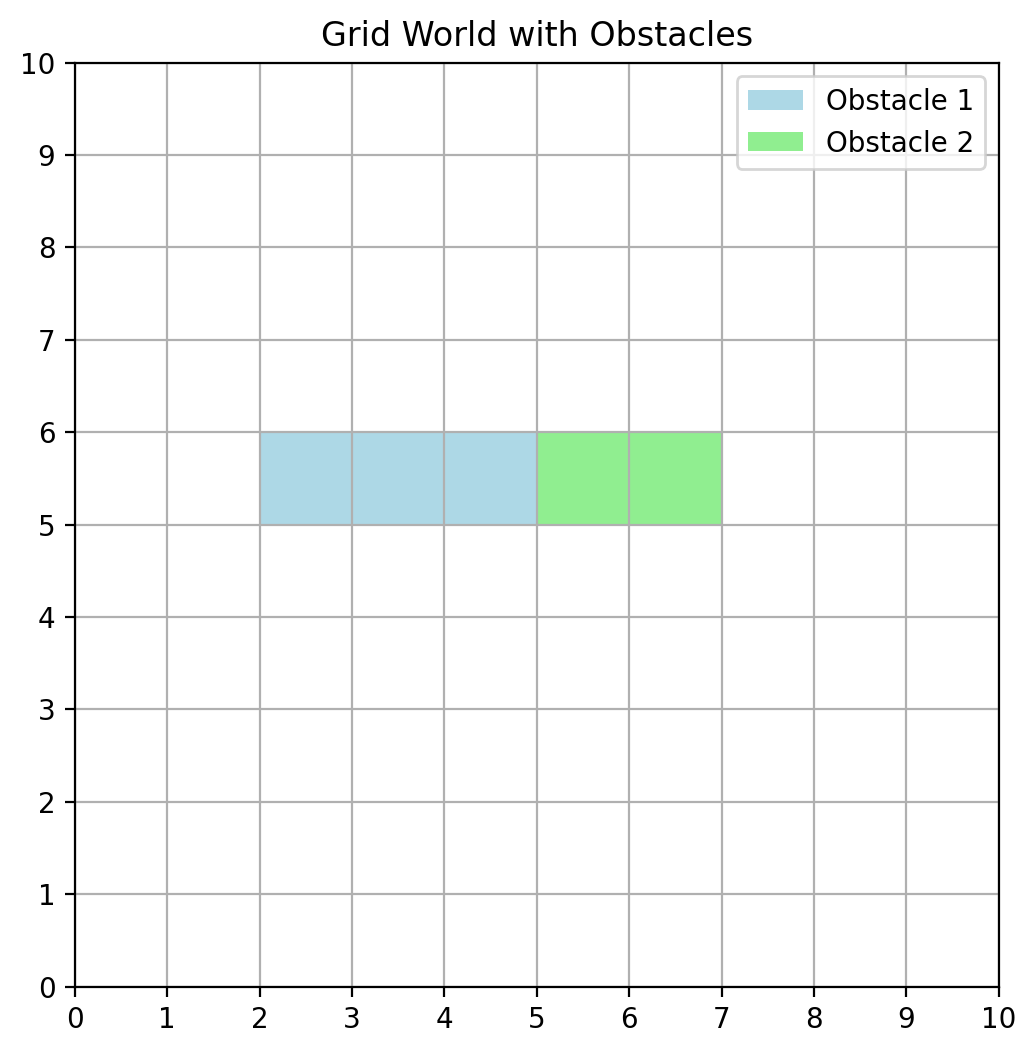
\includegraphics[width=\linewidth]{figures/world.png}
  \caption{The grid world.}
\end{subfigure}\hfill
\begin{subfigure}[t]{0.42\linewidth}
  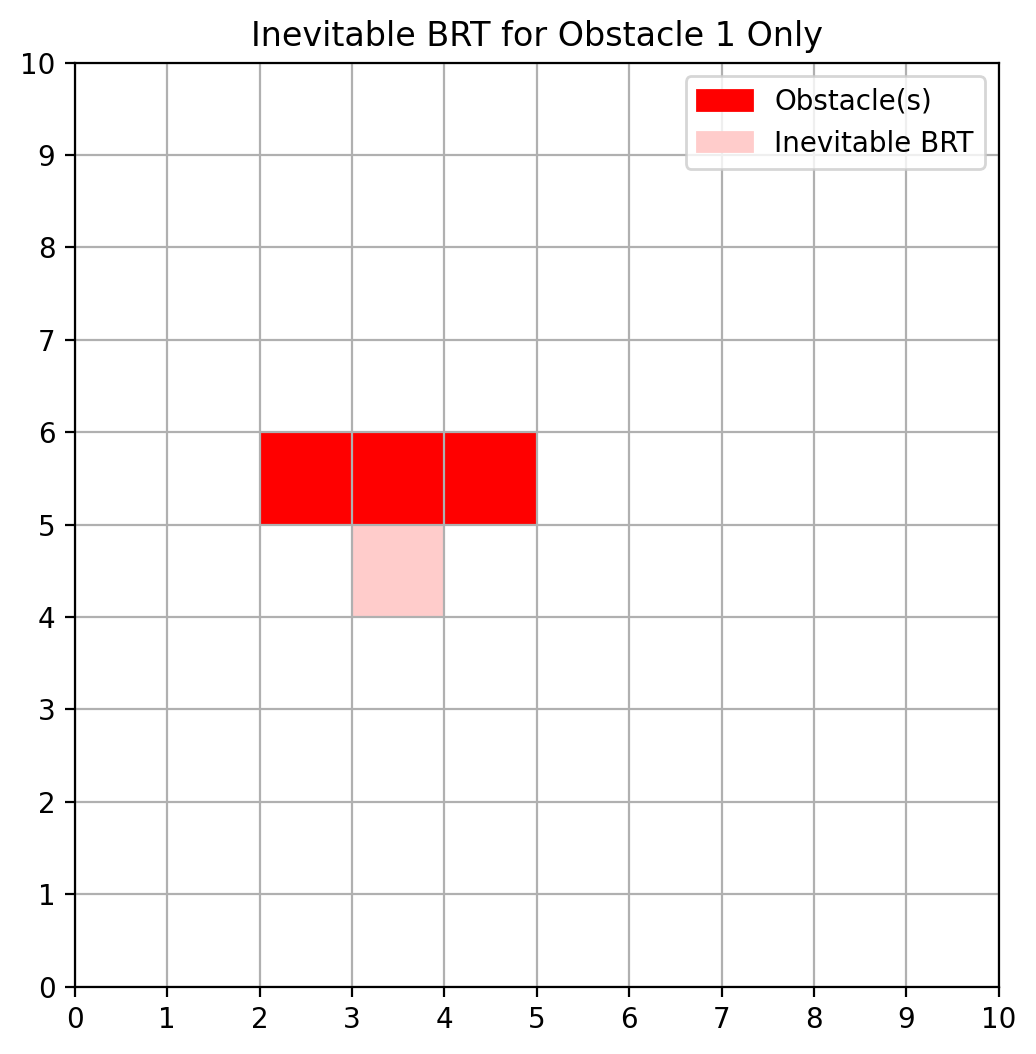
\includegraphics[width=\linewidth]{figures/brt_obstacle1.png}
  \caption{Obstacle 1 only.}
\end{subfigure}\\[2mm]
\begin{subfigure}[t]{0.42\linewidth}
  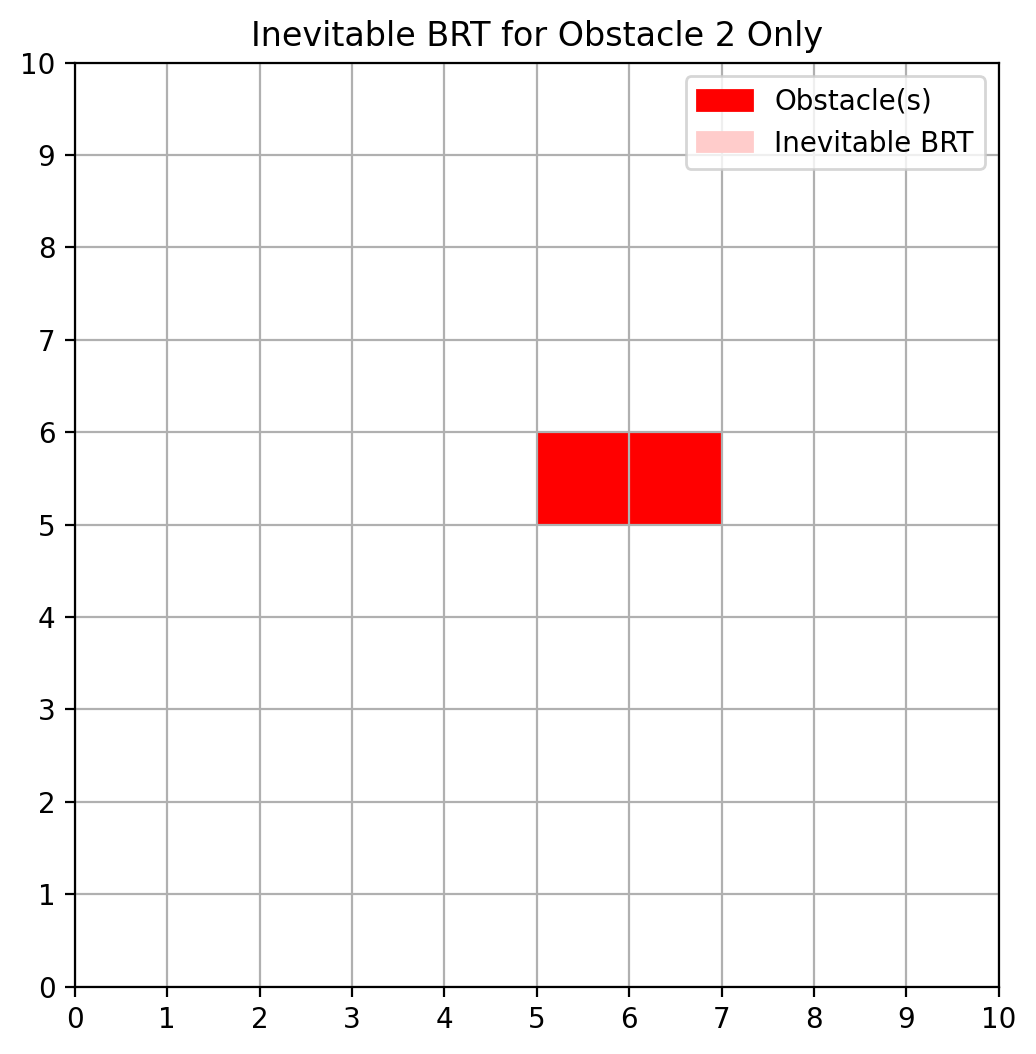
\includegraphics[width=\linewidth]{figures/brt_obstacle2.png}
  \caption{Obstacle 2 only.}
\end{subfigure}\hfill
\begin{subfigure}[t]{0.42\linewidth}
  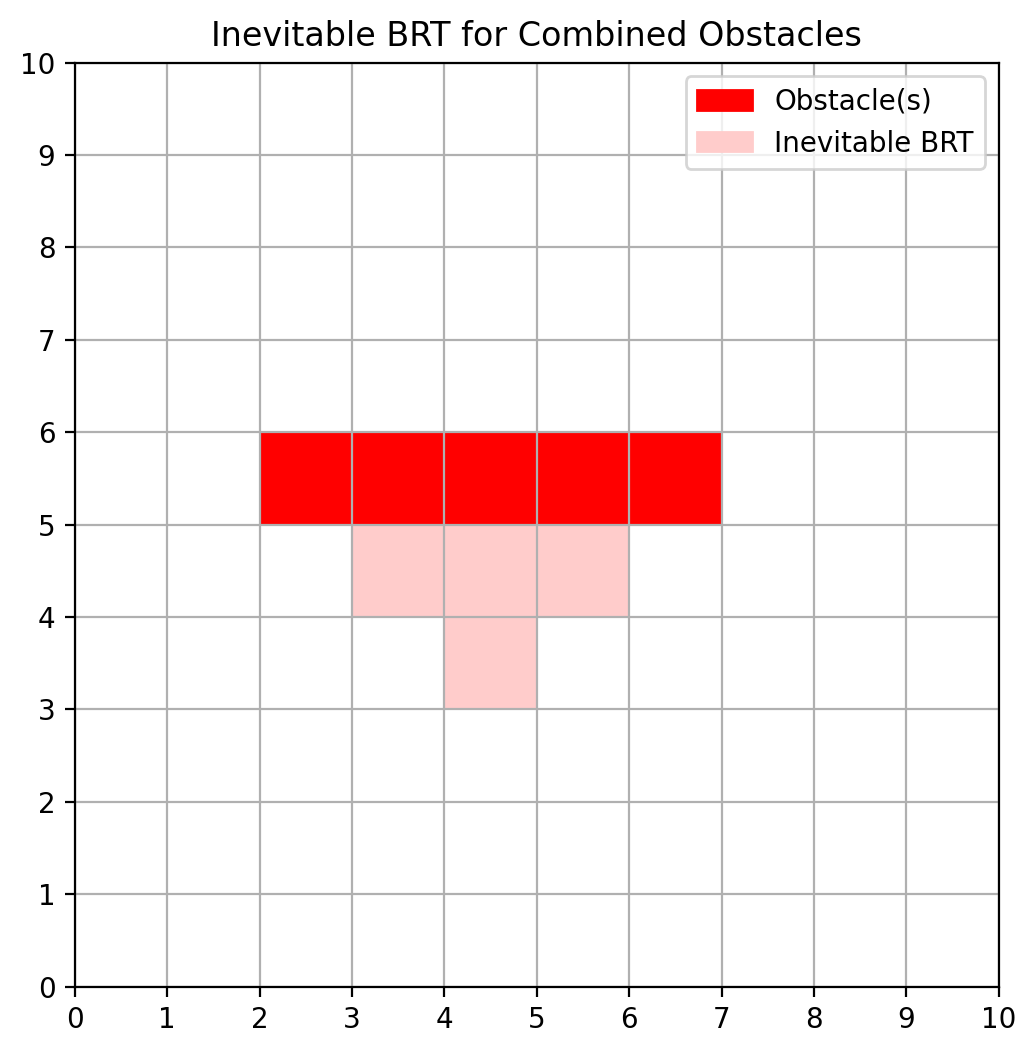
\includegraphics[width=\linewidth]{figures/brt_combined.png}
  \caption{Both obstacles.}
\end{subfigure}
\caption{Inevitable backward-reachable tubes (light red) of the obstacle sets (red).}
\label{fig:brt}
\end{figure}

\subsection*{Discussion}

\paragraph{Why the tubes look the way they do.}
The robot cannot stop or slow down, so a cell $d$ rows below the obstacle row will land on that row
after exactly $d$ steps, at a column anywhere in $\{x-d,\dots,x+d\}$ (any integer in that range is
attainable by an appropriate control sequence). Collision is inevitable if and only if
\emph{every} one of those landing columns is occupied, i.e.\ $\{x-d,\dots,x+d\}\subseteq$ obstacle
columns. For a contiguous obstacle of width $w$ this means $2d\le w-1$, so the tube is an inverted
triangle (a cone with unit slope) of height $\lfloor (w-1)/2\rfloor$ below the obstacle's centre:
height $1$ for the width-3 obstacle, height $0$ for the width-2 obstacle, and height $2$ for the
combined width-5 obstacle. This is exactly what the code produces, and it matches intuition: since
the robot's lateral speed equals its forward speed, it can escape any obstacle whose half-width is
smaller than its current distance to the obstacle row, so the doomed region hugs the obstacle
tightly. Everything above the obstacle row and everything in the rows below it that is outside the
cone is safe. Note that the width-2 obstacle alone has an empty tube beyond itself: from $(5,4)$ or
$(6,4)$ the robot can always step to a free neighbouring column.

\paragraph{Combined obstacles versus the union of the individual tubes.}
The union of the two individual tubes adds only $(3,4)$ to the obstacle cells, whereas the tube of
the combined failure set adds $(3,4)$, $(4,4)$, $(5,4)$ and $(4,3)$ (Figure~\ref{fig:union}). The
combined tube \emph{strictly contains} the union. The extra cells are states from which every escape
from one obstacle lands in the other: from $(4,4)$, steering left or going straight hits obstacle~1
while steering right hits obstacle~2, and from $(4,3)$ all three successors are among these doomed
cells. This is the discrete version of Problem~1.2(c): a state can be safe with respect to
$\failure_1$ and safe with respect to $\failure_2$ using two \emph{different} controllers, yet unsafe
with respect to $\failure_1\cup\failure_2$, i.e.\
$\safeset(\failure_1\cup\failure_2)\subsetneq\safeset(\failure_1)\cap\safeset(\failure_2)$ and,
equivalently, $\inevitable{\backward{\reach}}(\failure_1\cup\failure_2)\supsetneq
\inevitable{\backward{\reach}}(\failure_1)\cup\inevitable{\backward{\reach}}(\failure_2)$. The
practical lesson is that safety analysis must be carried out on the \emph{full} failure set;
per-obstacle tubes cannot simply be unioned, and a ``harmless'' obstacle (obstacle~2 alone traps
nothing) can enlarge the unsafe region substantially once it sits next to another one. The boundary
of the tube is also where a least-restrictive safety filter would have to intervene: from $(3,3)$
the only safe action is $\ctrl=-1$, so the filter must override $\ctrl\in\{0,+1\}$ there, while it
can leave the controller free anywhere outside the tube.

\begin{figure}[h]
\centering
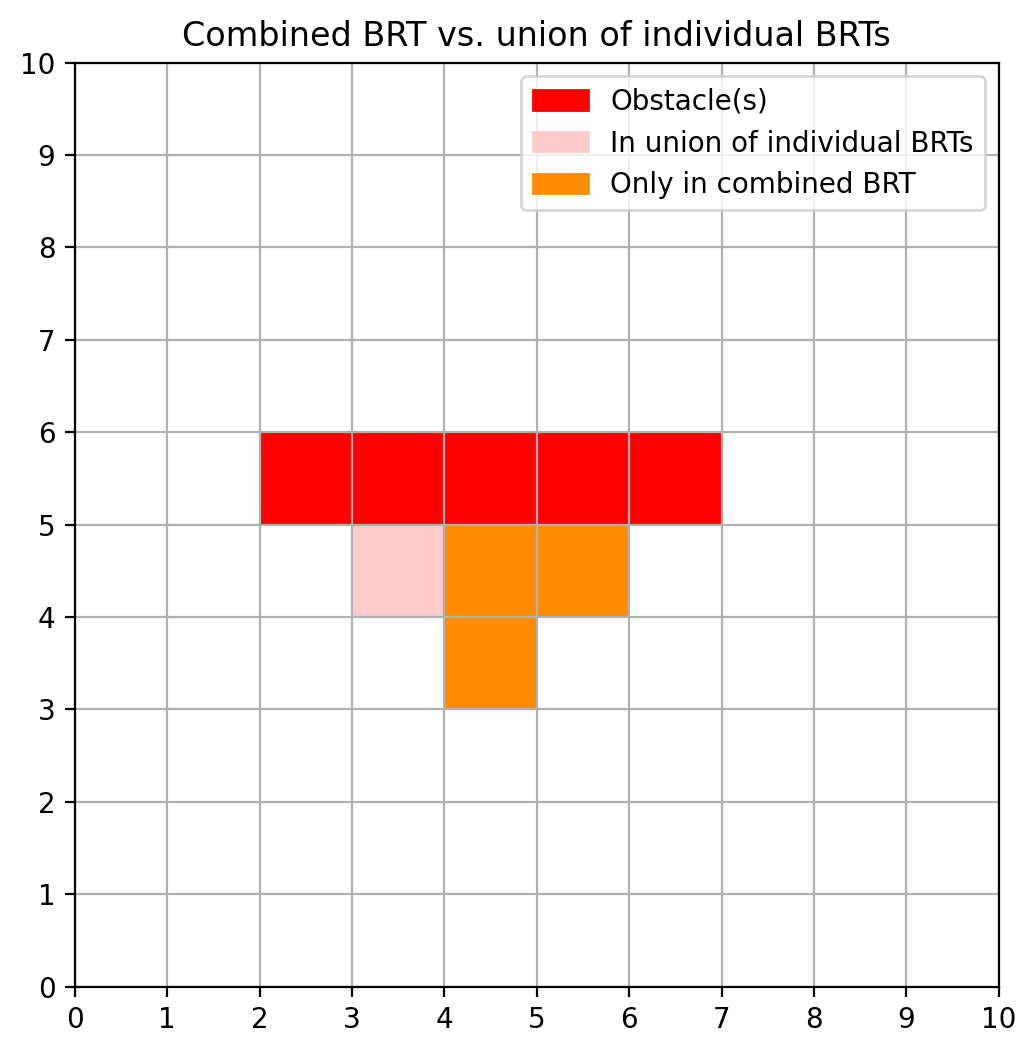
\includegraphics[width=0.42\linewidth]{figures/brt_union_vs_combined.png}
\caption{The tube of the combined failure set. Light red cells also belong to the union of the two
individual tubes; orange cells belong only to the combined tube.}
\label{fig:union}
\end{figure}

\paragraph{Effect of the forward-to-lateral speed ratio.}
The shape of the tube is set by the ratio of lateral to forward speed. If the robot advanced $v$
rows per step while still shifting by at most one column (equivalently, it could steer only once
every $v$ rows), then from $d$ rows away it could only reach columns within $\pm d/v$ of its current
one, and the trapping condition becomes $2d/v\le w-1$: the cone becomes steeper and its height grows
to about $v(w-1)/2$, so the inevitable tube \emph{grows}. A faster robot has fewer steps in which to
swerve, and in the limit of very fast forward motion every cell in the obstacle's ``shadow''
directly below it becomes doomed. Conversely, more lateral authority ($\ctrl\in\{-k,\dots,k\}$)
flattens the cone to height $\lfloor (w-1)/(2k)\rfloor$; with $k=2$ the combined tube would shrink to
the obstacles plus the single cell $(4,4)$, and obstacle~1's tube would shrink to the obstacle itself.
(In the literal discrete model a speed of $v=2$ rows per step also introduces a parity effect: a
robot starting on an even row would hop over the single obstacle row entirely, since grazing is
allowed. The statement above should therefore be read in the fine-grid or continuous-time limit,
where the obstacle has finite thickness.)

% If you are citing any references, you can use the standard bibliography below.
\bibliographystyle{IEEEtran}
\bibliography{references}  % Comment out if not including a bibliography.

\end{document}
